\begin{center}
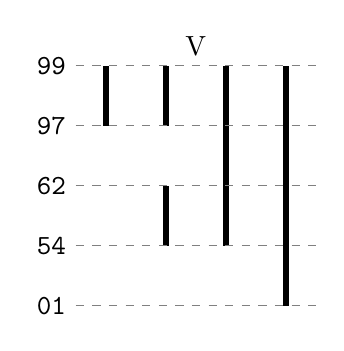
\begin{tikzpicture}[x=0.3in,y=0.3in]
\fill[white] (0,0) rectangle (3,4);
\draw[line width=2pt] (0,3) -- (0,4); 
\draw[line width=2pt] (1,1) -- (1,2); \draw[line width=2pt] (1,3) -- (1,4); 
\draw[line width=2pt] (2,1) -- (2,4);
\draw[line width=2pt] (3,0) -- (3,4); 
\node[above] at (1.5,4) {V};
\node[left] at (-0.5,0) {\tt01};
\node[left] at (-0.5,1) {\tt54};
\node[left] at (-0.5,2) {\tt62};
\node[left] at (-0.5,3) {\tt97};
\node[left] at (-0.5,4) {\tt99};
\foreach \y in {0,1,2,3,4} {
\draw[dashed,black!50] (-0.5,\y) -- (3.5,\y);
}
\end{tikzpicture}
\hspace{1em}
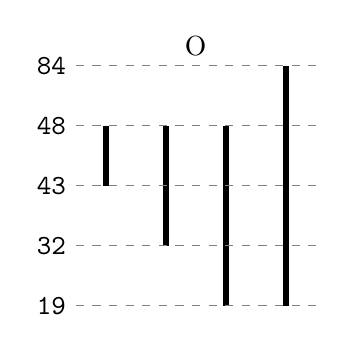
\begin{tikzpicture}[x=0.3in,y=0.3in]
\fill[white] (0,0) rectangle (3,4);
\draw[line width=2pt] (0,2) -- (0,3); 
\draw[line width=2pt] (1,1) -- (1,3);
\draw[line width=2pt] (2,0) -- (2,3); 
\draw[line width=2pt] (3,0) -- (3,4); 
\node[above] at (1.5,4) {O};
\node[left] at (-0.5,0) {\tt19};
\node[left] at (-0.5,1) {\tt32};
\node[left] at (-0.5,2) {\tt43};
\node[left] at (-0.5,3) {\tt48};
\node[left] at (-0.5,4) {\tt84};
\foreach \y in {0,1,2,3,4} {
\draw[dashed,black!50] (-0.5,\y) -- (3.5,\y);
}
\end{tikzpicture}
\hspace{1em}
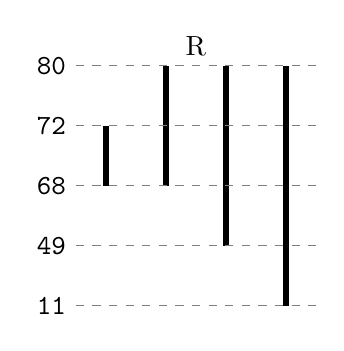
\begin{tikzpicture}[x=0.3in,y=0.3in]
\fill[white] (0,0) rectangle (3,4);
\draw[line width=2pt] (0,2) -- (0,3); 
\draw[line width=2pt] (1,2) -- (1,4); 
\draw[line width=2pt] (2,1) -- (2,4);
\draw[line width=2pt] (3,0) -- (3,4); 
\node[above] at (1.5,4) {R};
\node[left] at (-0.5,0) {\tt11};
\node[left] at (-0.5,1) {\tt49};
\node[left] at (-0.5,2) {\tt68};
\node[left] at (-0.5,3) {\tt72};
\node[left] at (-0.5,4) {\tt80};
\foreach \y in {0,1,2,3,4} {
\draw[dashed,black!50] (-0.5,\y) -- (3.5,\y);
}
\end{tikzpicture}

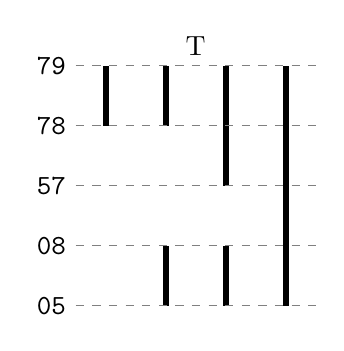
\begin{tikzpicture}[x=0.3in,y=0.3in]
\fill[white] (0,0) rectangle (3,4);
\draw[line width=2pt] (0,3) -- (0,4); 
\draw[line width=2pt] (1,0) -- (1,1); \draw[line width=2pt] (1,3) -- (1,4); 
\draw[line width=2pt] (2,0) -- (2,1); \draw[line width=2pt] (2,2) -- (2,4); 
\draw[line width=2pt] (3,0) -- (3,4); 
\node[above] at (1.5,4) {T};
\node[left] at (-0.5,0) {\tt05};
\node[left] at (-0.5,1) {\tt08};
\node[left] at (-0.5,2) {\tt57};
\node[left] at (-0.5,3) {\tt78};
\node[left] at (-0.5,4) {\tt79};
\foreach \y in {0,1,2,3,4} {
\draw[dashed,black!50] (-0.5,\y) -- (3.5,\y);
}
\end{tikzpicture}
\hspace{1em}
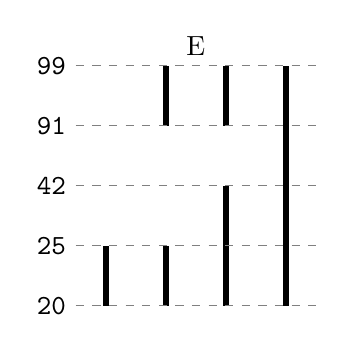
\begin{tikzpicture}[x=0.3in,y=0.3in]
\fill[white] (0,0) rectangle (3,4);
\draw[line width=2pt] (0,0) -- (0,1); 
\draw[line width=2pt] (1,0) -- (1,1); \draw[line width=2pt] (1,3) -- (1,4); 
\draw[line width=2pt] (2,0) -- (2,2); \draw[line width=2pt] (2,3) -- (2,4); 
\draw[line width=2pt] (3,0) -- (3,4); 
\node[above] at (1.5,4) {E};
\node[left] at (-0.5,0) {\tt20};
\node[left] at (-0.5,1) {\tt25};
\node[left] at (-0.5,2) {\tt42};
\node[left] at (-0.5,3) {\tt91};
\node[left] at (-0.5,4) {\tt99};
\foreach \y in {0,1,2,3,4} {
\draw[dashed,black!50] (-0.5,\y) -- (3.5,\y);
}
\end{tikzpicture}
\hspace{1em}
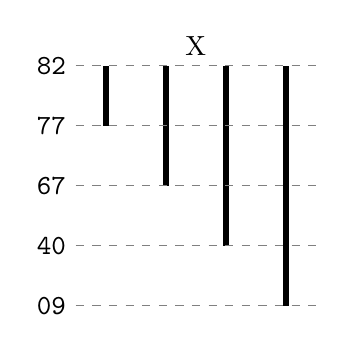
\begin{tikzpicture}[x=0.3in,y=0.3in]
\fill[white] (0,0) rectangle (3,4);
\draw[line width=2pt] (0,3) -- (0,4); 
\draw[line width=2pt] (1,2) -- (1,4);
\draw[line width=2pt] (2,1) -- (2,4);
\draw[line width=2pt] (3,0) -- (3,4); 
\node[above] at (1.5,4) {X};
\node[left] at (-0.5,0) {\tt09};
\node[left] at (-0.5,1) {\tt40};
\node[left] at (-0.5,2) {\tt67};
\node[left] at (-0.5,3) {\tt77};
\node[left] at (-0.5,4) {\tt82};
\foreach \y in {0,1,2,3,4} {
\draw[dashed,black!50] (-0.5,\y) -- (3.5,\y);
}
\end{tikzpicture}
\end{center}
